\chapter{Clustering}

This chapter describes clustering approaches using four different distance measures. Euclidean, DTW, Cosine and NCD.

For every approach the "heart rate" time series with a 5min granularity was used. The clustering was done with the k-Means algorithm.

Figure \ref{fig:all_ts_clust} shows all time series used for the clustering.



\begin{figure}[h!]
	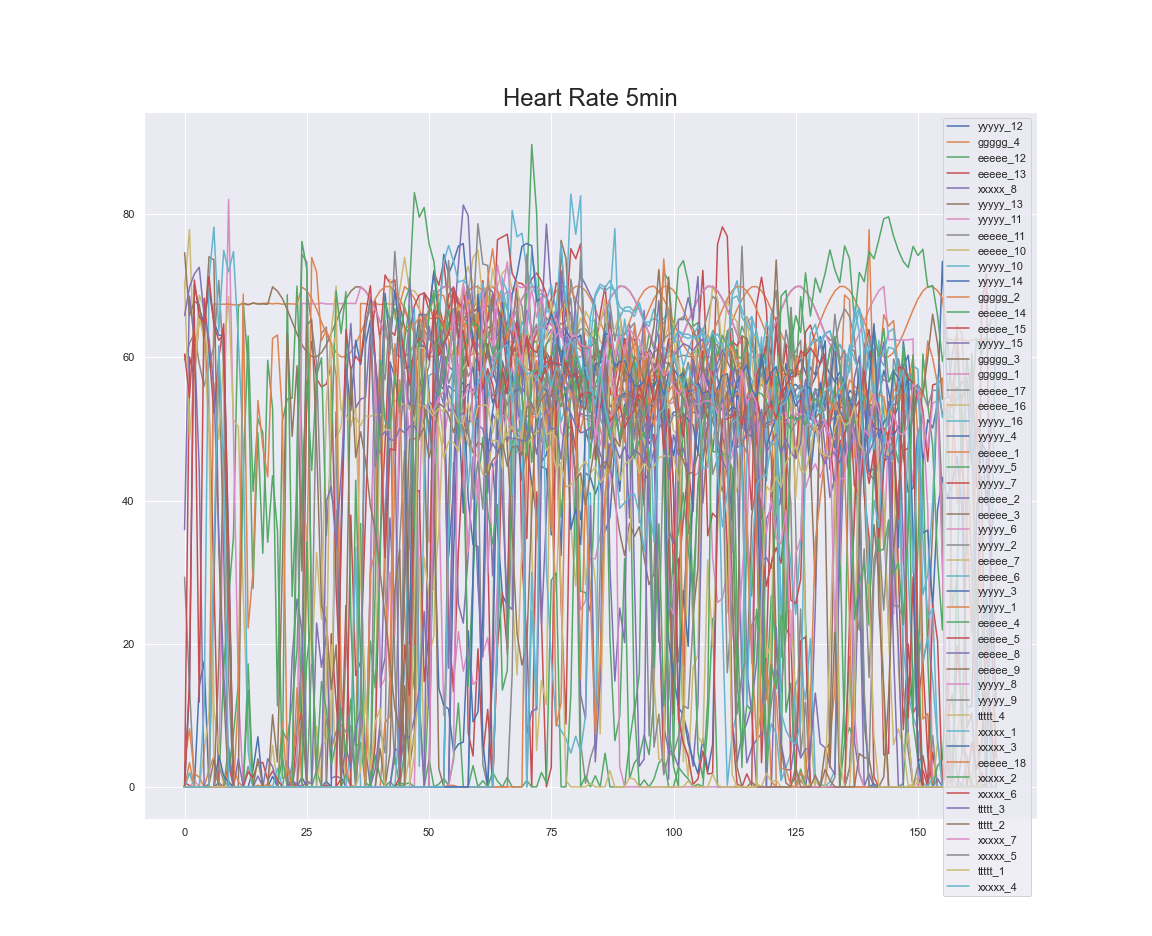
\includegraphics[width=1\textwidth]{hr_5min_all.png}
	\caption{All time series used for clustering}
	\label{fig:all_ts_clust}
\end{figure}

In order to calculate distances between the time series, they had to be normalized using the "z-score" standardisation.

$$ z = \frac{x - \mu}{\sigma} $$
$$ x : \text{Time Series} $$
$$ \mu: \text{Mean of the Time Series} $$
$$ \sigma: \text{Standard deviation of the time series} $$


Figure \ref{fig:all_ts_clust_normalized} shows all normalized time series.

\begin{figure}[h!]
	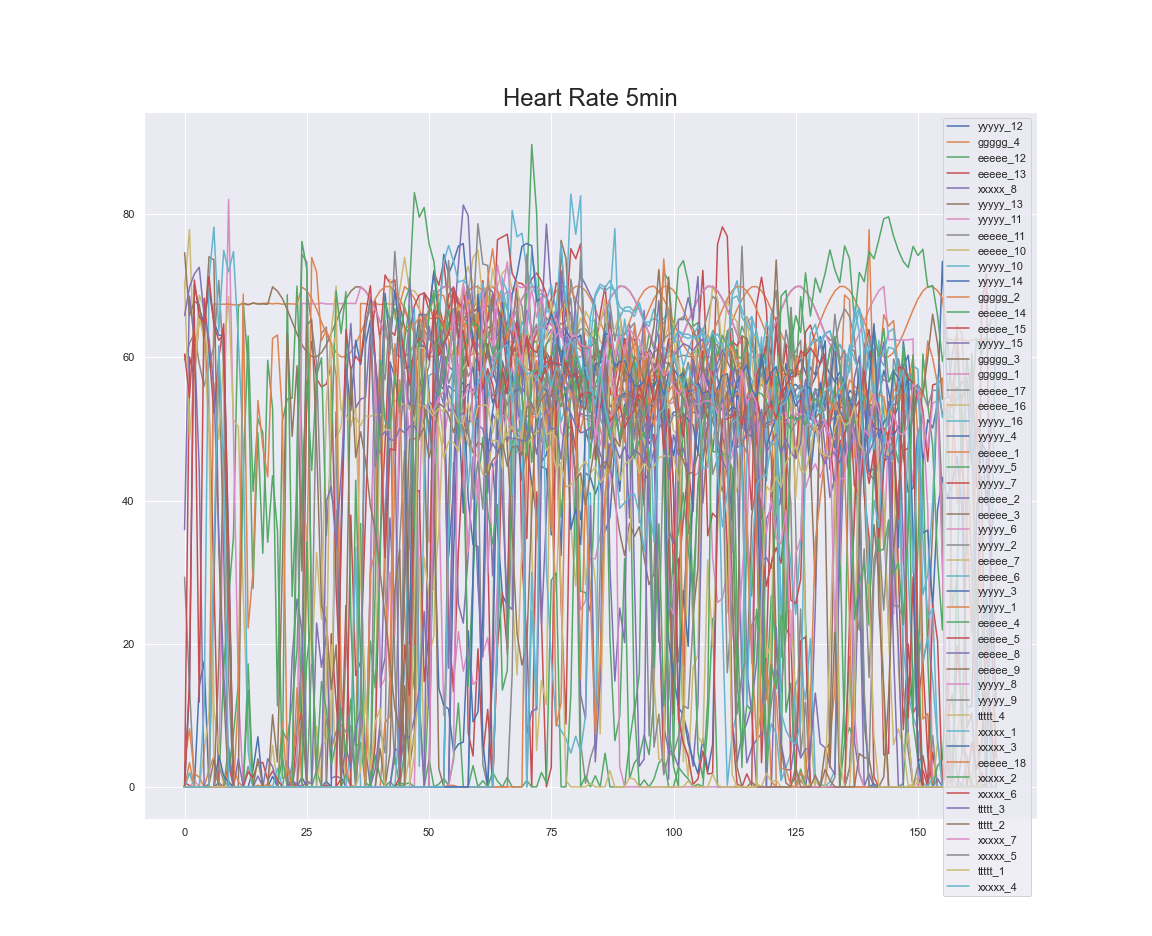
\includegraphics[width=1\textwidth]{hr_5min_all_normalized.png}
	\caption{All time series used for clustering normalized}
	\label{fig:all_ts_clust_normalized}
\end{figure}


%%%%%%%%%%%%%%%%%%%%%%%%%%%%%%%%%%%%%%%

\clearpage
\section{Using Euclidean Distance}

This chapter describes the clustering using Euclidean distances. The corresponding code can be found in \path{Clustering1_Euclidean.ipynb}.


Figure \ref{fig:cvi_euc} displays the four used CVIs as a function of number of clusters going from 2 to 20. The Calinski Harabasz score shows a nice "elbow". The other CVI functions however do not allow for the elbow-method to be applied.

\begin{figure}[h!]
	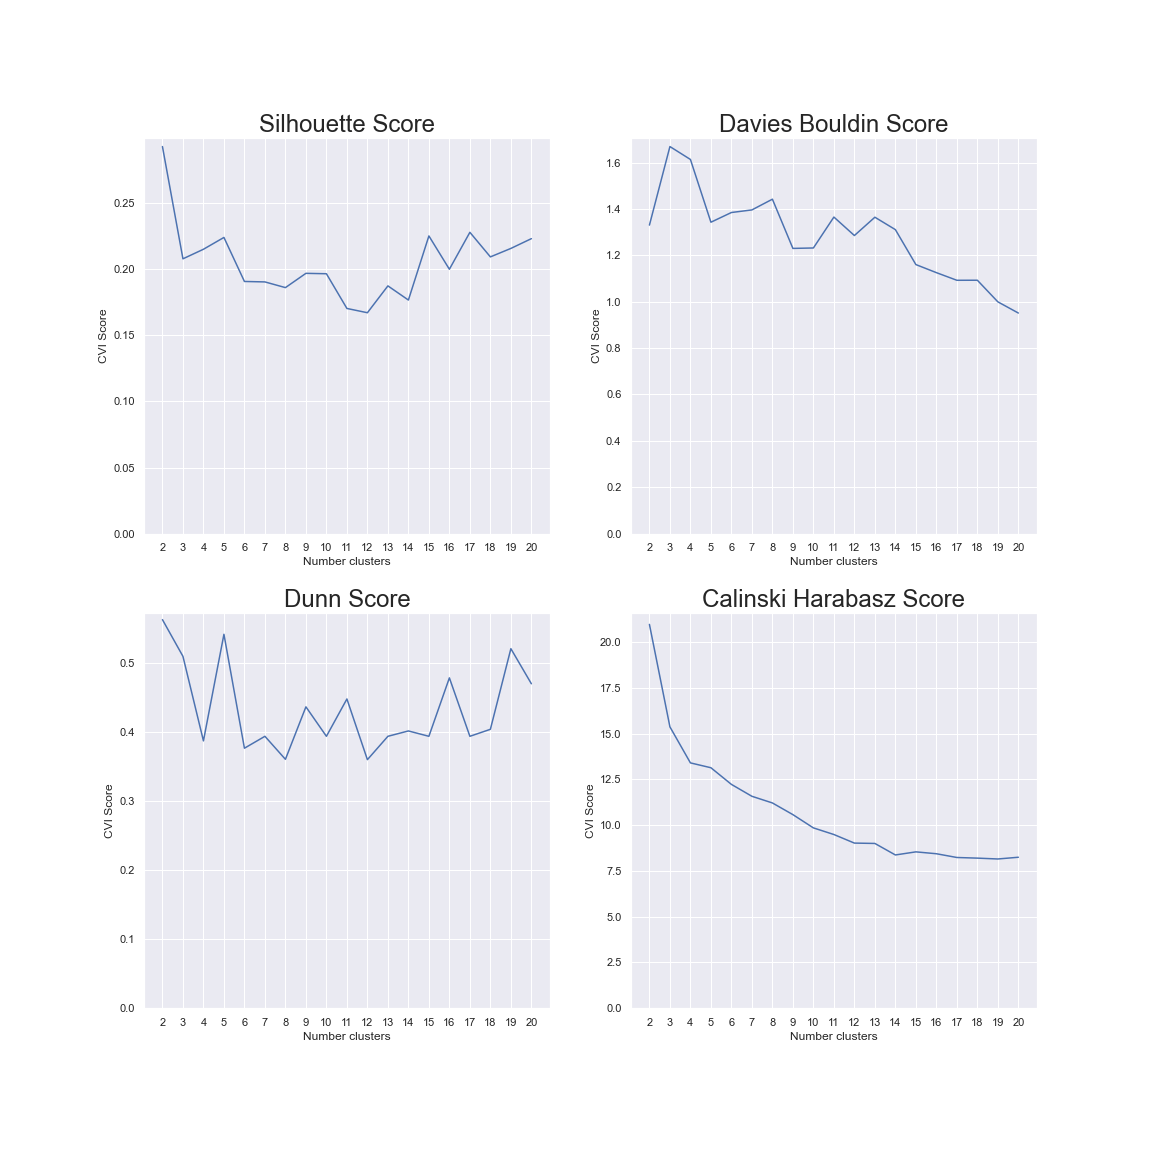
\includegraphics[width=1\textwidth]{euclidean_cvis.png}
	\caption{CVI Functions of Euclidean Distance}
	\label{fig:cvi_euc}
\end{figure}

\clearpage
Due to the difficulty of selecting the optimal amount of clusters, a custom algorithm has been written. The goal is to combine the CVI scores to one function, which then can be visualized. 
The DB score is inversed because, unlike the other scores, it optimal value is zero. Then all CVIs are normalized to have the same impact of the resulting function. At the end all normalized CVIs are sum up and returned. This later on helps to select a cluster amount with an overall good CVI-score.

The visualizazion of this function is displayed in figure \ref{fig:cvi_euc_combo}. The code for the algorithm is shown below.




\begin{lstlisting}[language=Python]
#!/usr/bin/env python
__author__  = "Yannis Schmutz"
__version__ = "0.1.0"
__email__   = "schmy3@bfh.ch"
__status__  = "Dev"

import numpy as np


def get_cvi_combination(*, sil, dunn, db, ch):
    # Transform cvi values to numpy arrays
    sil_values = np.array(sil)
    dunn_values = np.array(dunn)
    ch_values = np.array(ch)	
    # Inverse db-score (we want to maximise the cvi-combination)
    db_inv_values = np.array(list(map(lambda v: 1/v, db)))
	
    # Normalize cvis in order to have an equal impact
    sil_mean = sil_values.mean()
    sil_std = sil_values.std()

    dunn_mean = dunn_values.mean()
    dunn_std = dunn_values.std()

    ch_mean = ch_values.mean()
    ch_std = ch_values.std()

    db_inv_mean = db_inv_values.mean()
    db_inv_std = db_inv_values.std()

    sil_n_values = (sil_values - sil_mean) / sil_std
    dunn_n_values = (dunn_values - dunn_mean) / dunn_std
    ch_n_values = (ch_values - ch_mean) / ch_std
    db_inv_n_values = (db_inv_values - db_inv_mean) / db_inv_std
	
    # Summ up all cvis
    combination = sil_n_values + dunn_n_values + db_inv_n_values + ch_n_values
    return combination

\end{lstlisting}

\clearpage
Given the combination of all CVIs, 16 seems like a reasonable number of clusters to use.

\begin{figure}[h!]
	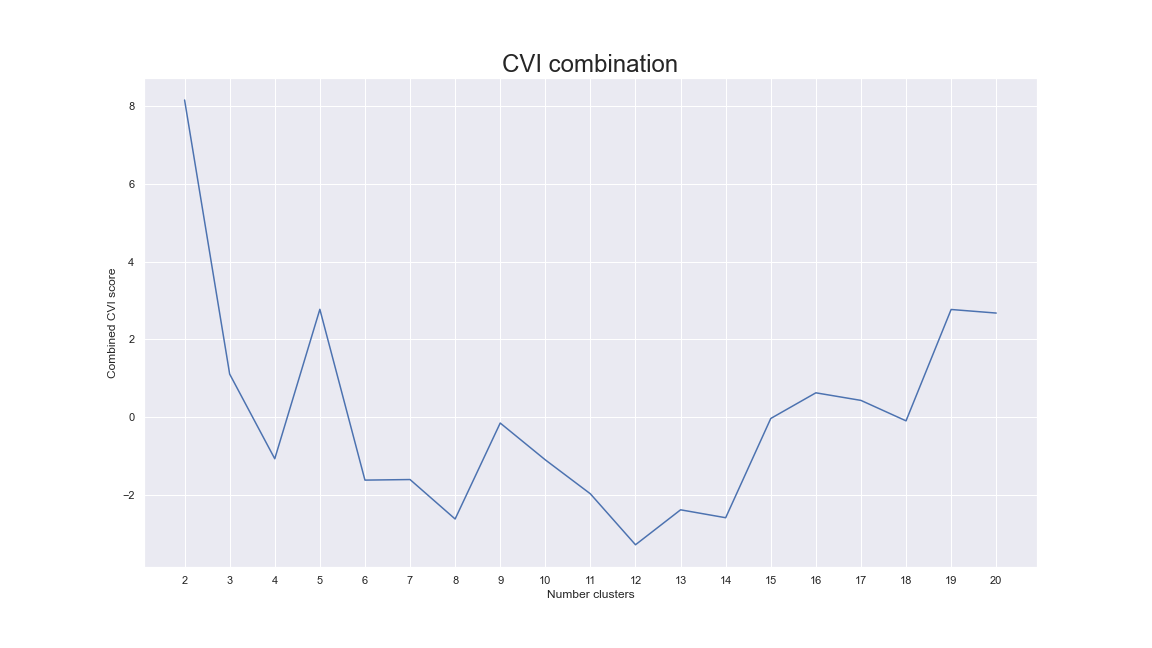
\includegraphics[width=1\textwidth]{cvi_combination_euc.png}
	\caption{CVI Combination (Euclidean Distance)}
	\label{fig:cvi_euc_combo}
\end{figure}


\clearpage
Figure \ref{fig:euc_clusters} shows the outcome of the k-Means algorithm using 16 clusters. 11 of them contain only sleeping data from the same probant. Cluster \#8 and \#11 only contain one time series. This is due to their much different shape compared to "normal" sleeping behaviour.

\begin{figure}[h!]
	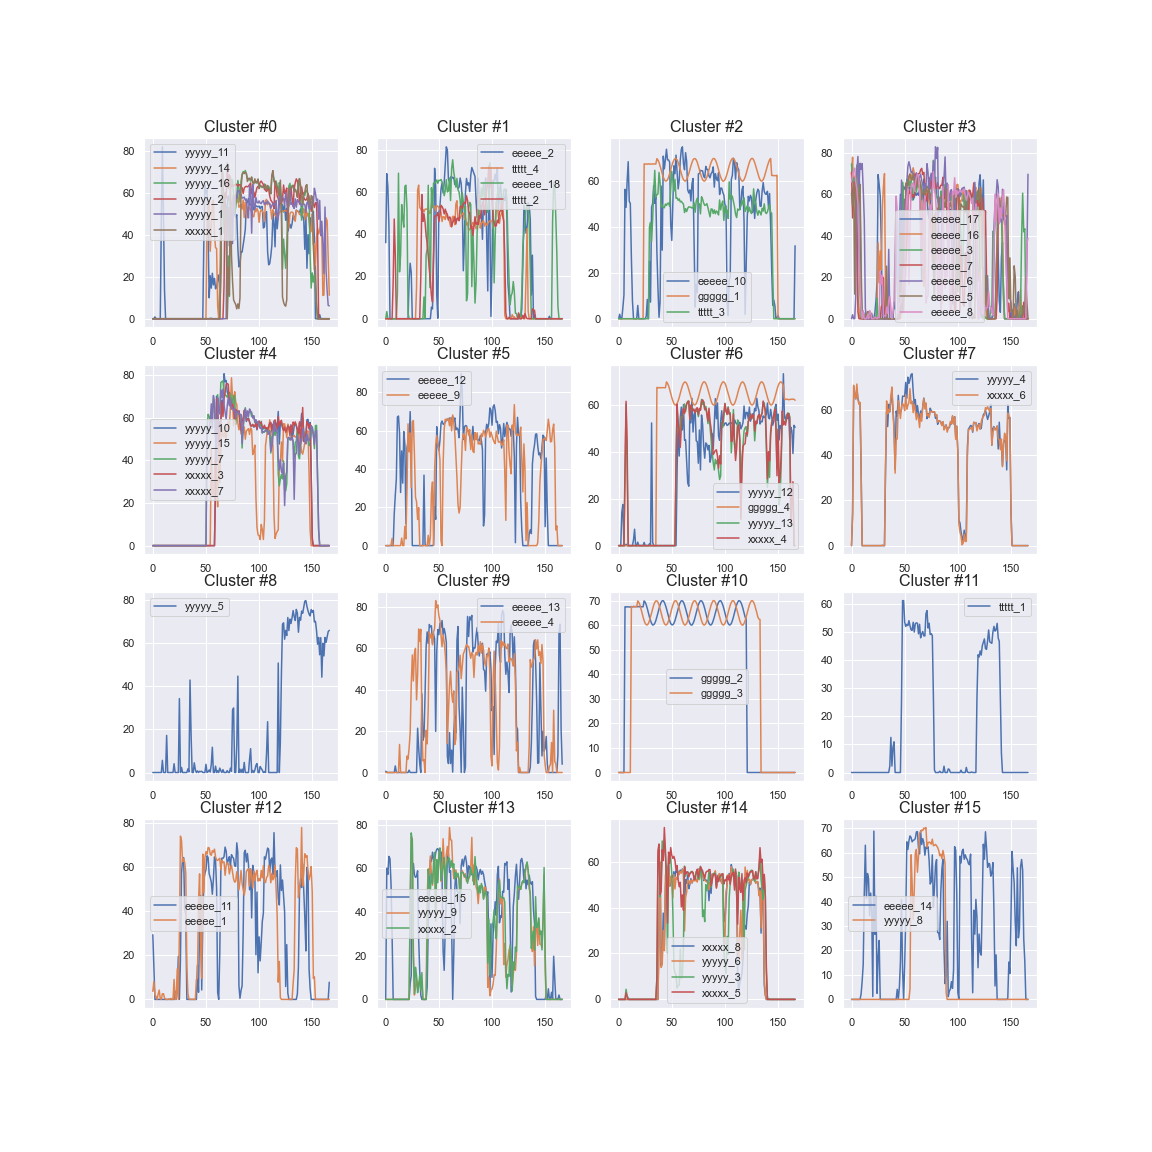
\includegraphics[width=1.1\textwidth]{euclidean_clustering.png}
	\caption{Clusters (Euclidean Distance)}
	\label{fig:euc_clusters}
\end{figure}


%%%%%%%%%%%%%%%%%%%%%%%%%%%%%%%%%%%%%%%

\clearpage
\section{Dynamic Time Warping}

This chapter describes the clustering using DTW distances. The corresponding code can be found in \path{Clustering2_DTW.ipynb}.


Figure \ref{fig:cvi_dtw} shows the four used CVIs as a function of number of clusters going from 2 to 20. None of the CVIs has a nice "elbow". Therefore $k$ is chosen using the combination of all CVIs shown in figure \ref{fig:cvi_dtw_combo}

\begin{figure}[h!]
	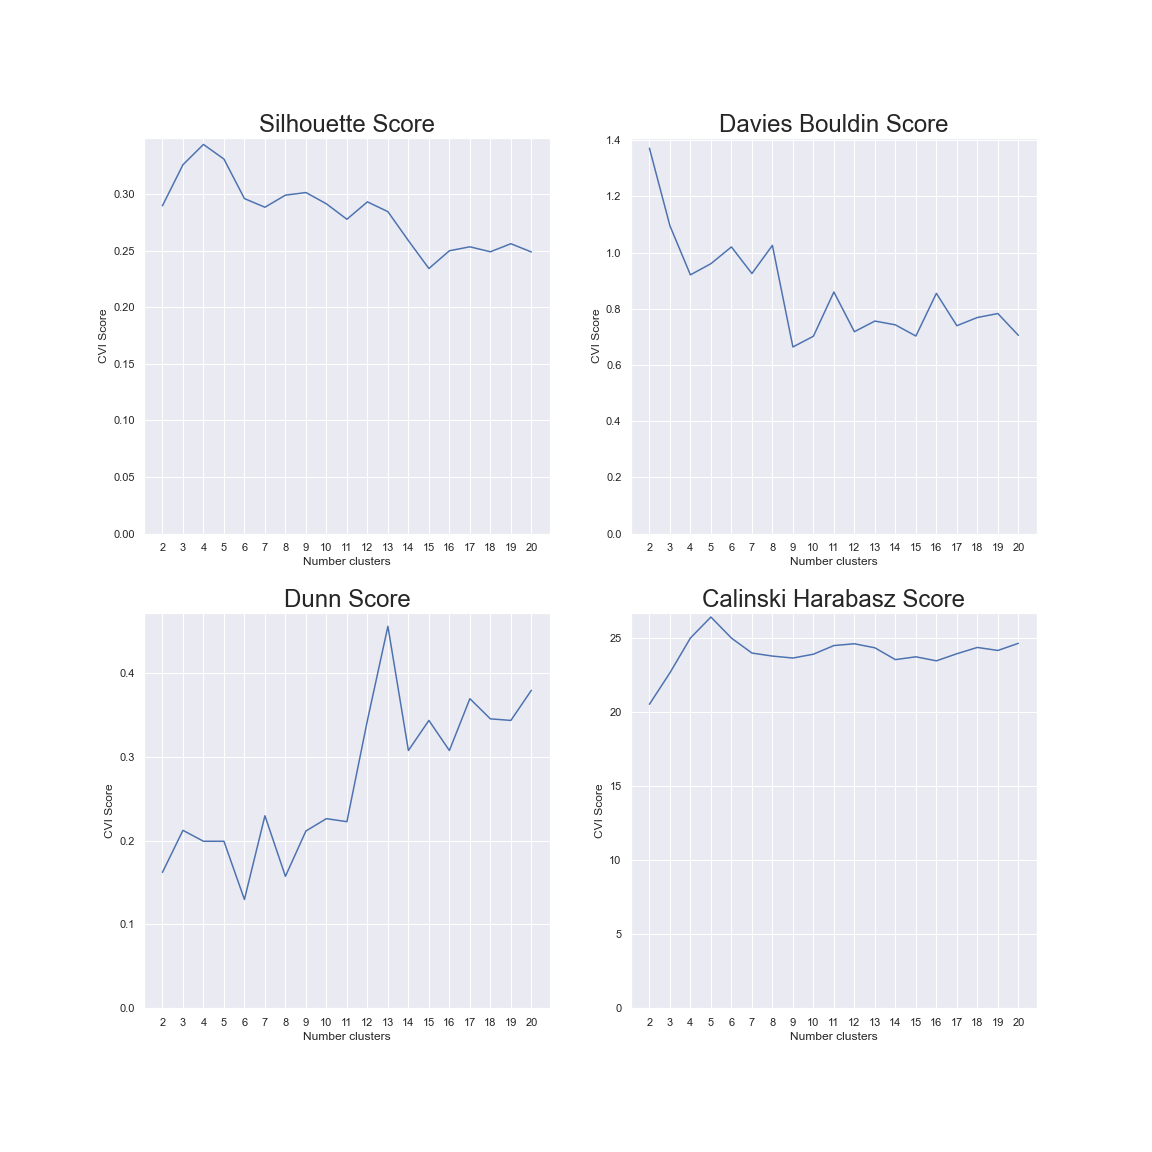
\includegraphics[width=1\textwidth]{dtw_cvis.png}
	\caption{CVI Functions of DTW Distance}
	\label{fig:cvi_dtw}
\end{figure}

\clearpage
13 clusters results in the highest overall CVI score and is therefore chosen for $k$.

\begin{figure}[h!]
	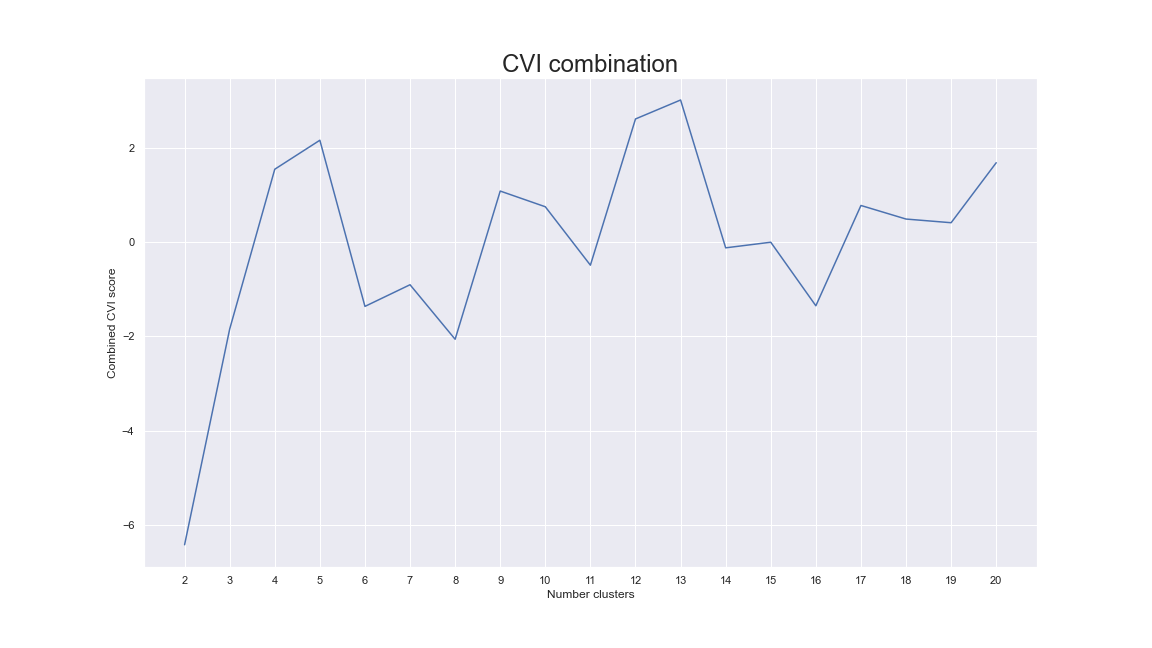
\includegraphics[width=1\textwidth]{cvi_combination_dtw.png}
	\caption{CVI Combination (DTW)}
	\label{fig:cvi_dtw_combo}
\end{figure}


\clearpage
Figure \ref{fig:dtw_clusters} shows the outcome of the k-Means algorithm using 13 clusters.
Using DTW there now are 5 clusters containing only one time series each. It would be nice, if the time series yyyyy\_5, yyyyy\_8 and ttttt\_1 would be clustered together due to their noticeable different sleeping behaviour.

\begin{figure}[h!]
	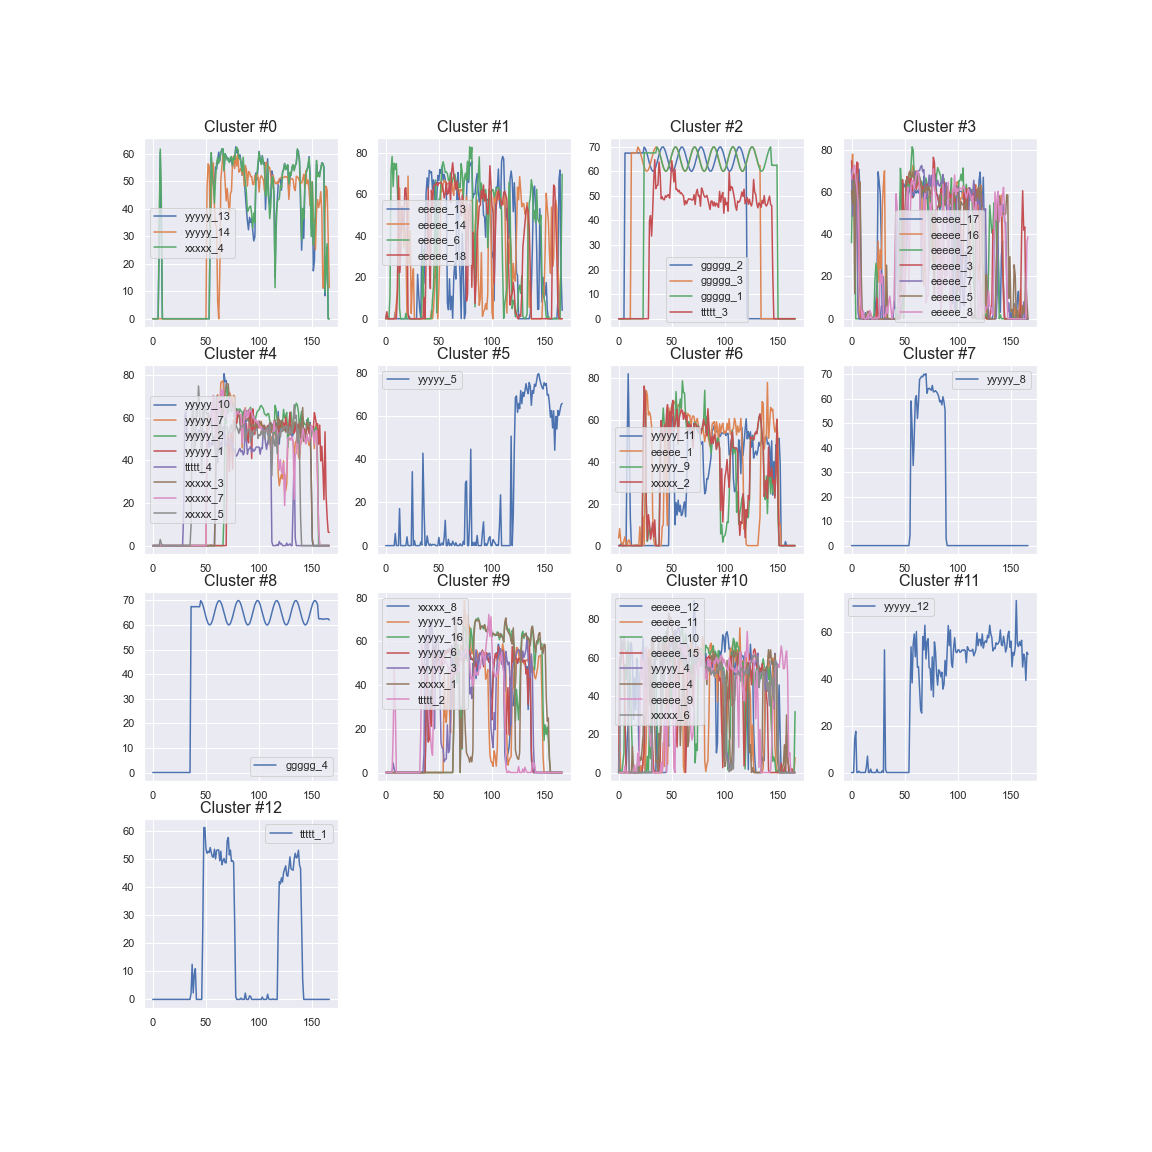
\includegraphics[width=1.1\textwidth]{dtw_clustering.png}
	\caption{Clusters (DTW Distance)}
	\label{fig:dtw_clusters}
\end{figure}

%%%%%%%%%%%%%%%%%%%%%%%%%%%%%%%%%%%%%%%

\clearpage
\section{Cosine}


This chapter describes the clustering using Cosine distances. The corresponding code can be found in \path{Clustering3_Cosine.ipynb}.


Figure \ref{fig:cvi_cosine} shows the four used CVIs as a function of number of clusters going from 2 to 20. The Calinski Harabasz graph resembles a little bit an elbow but is clearly not convincing enough to choose a $k$.


\begin{figure}[h!]
	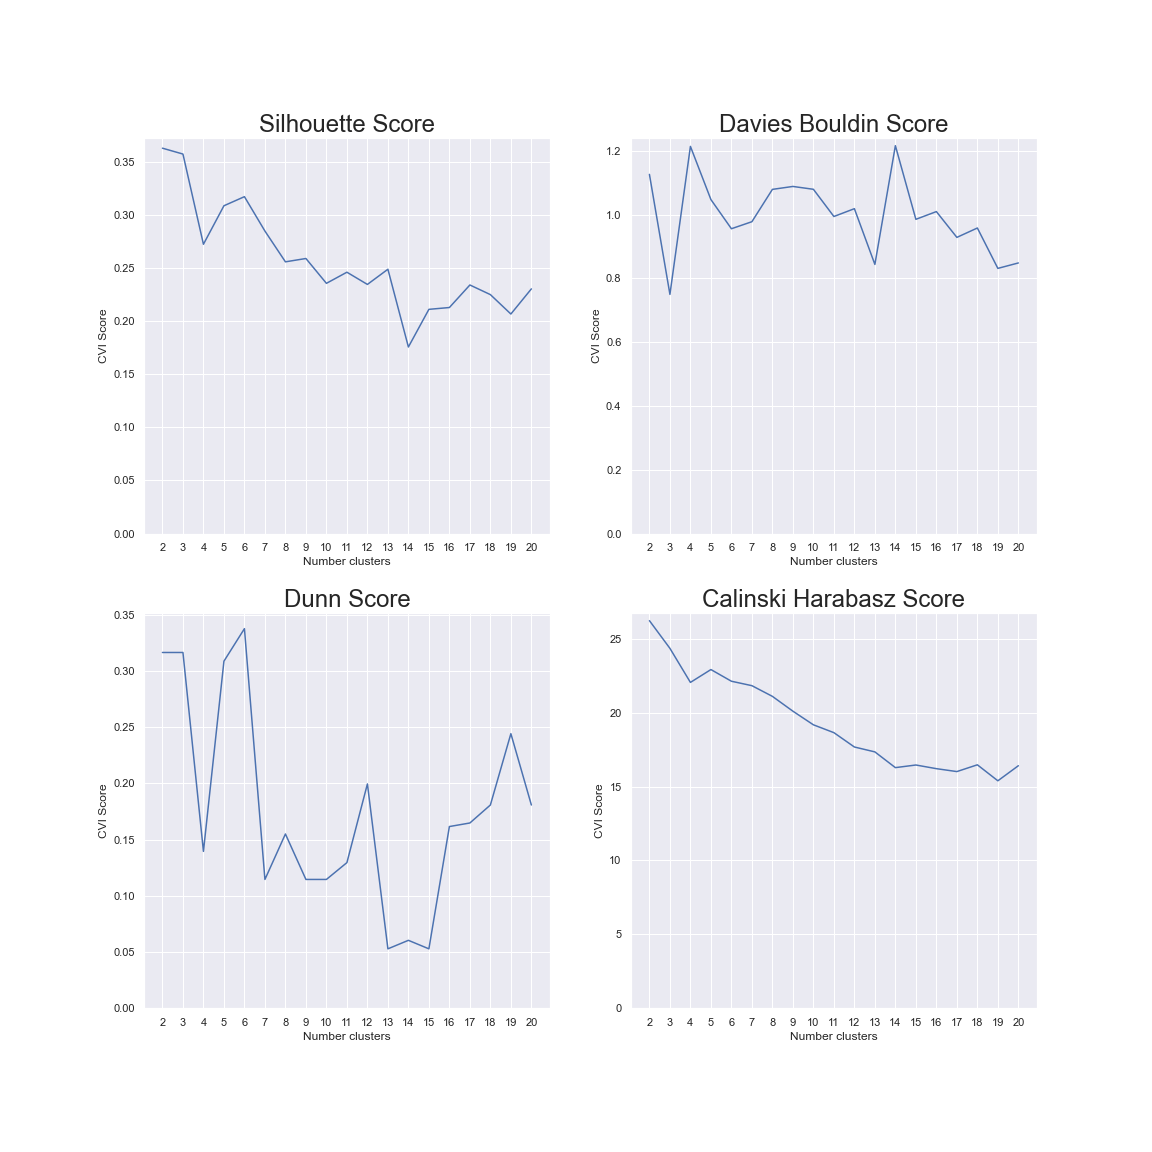
\includegraphics[width=1\textwidth]{cosine_cvis.png}
	\caption{CVI Functions of Cosine Distance}
	\label{fig:cvi_cosine}
\end{figure}


\clearpage
Even \ref{fig:cvi_cosine_combo} does not suggest a clear choice of $k$. Therefore different number of clusters between 6 and 13 had been tried out. 12 clusters had been found the best solution, which is shown in figure \ref{fig:cosine_clusters}.

\begin{figure}[h!]
	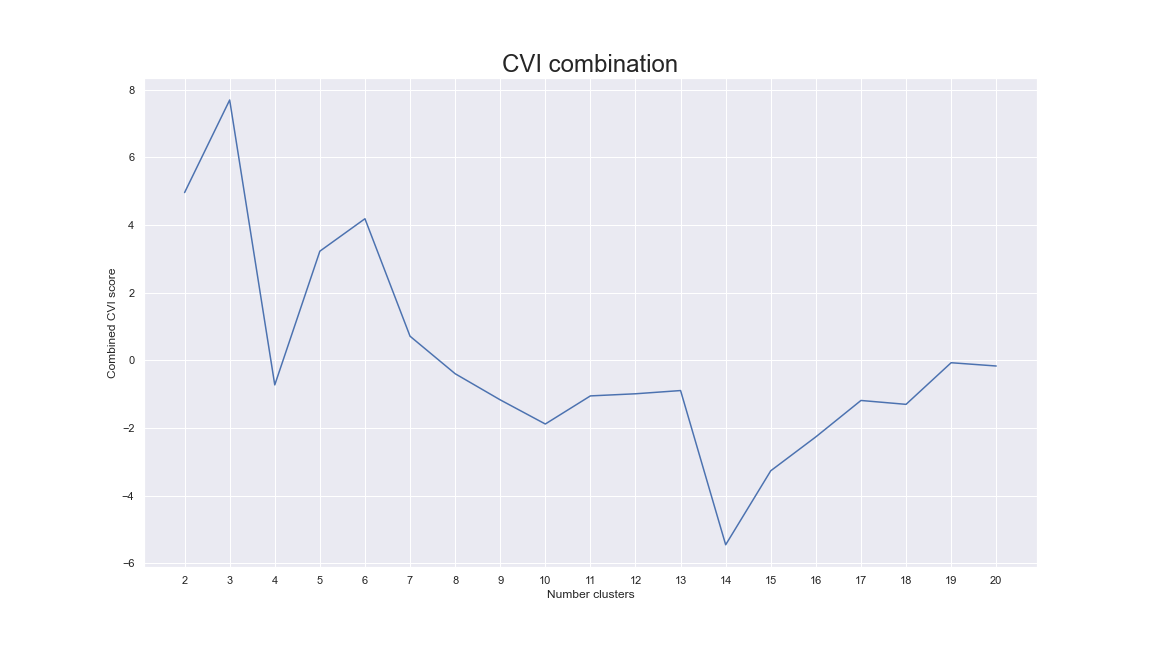
\includegraphics[width=1\textwidth]{cvi_combination_cosine.png}
	\caption{CVI Combination (Cosine)}
	\label{fig:cvi_cosine_combo}
\end{figure}

\clearpage
\begin{figure}[h!]
	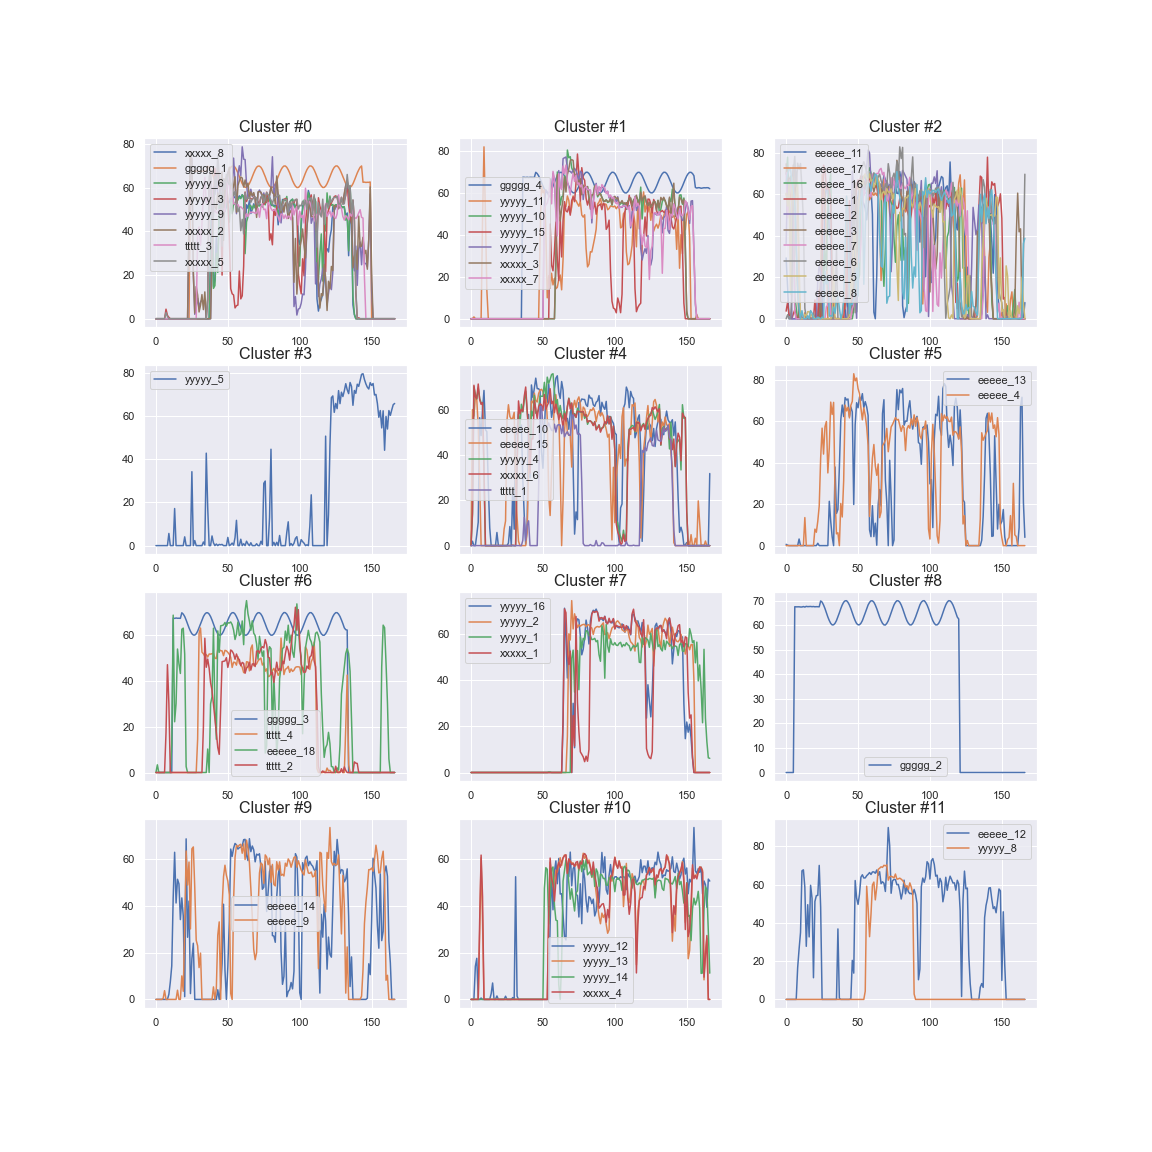
\includegraphics[width=1.1\textwidth]{cosine_clustering.png}
	\caption{Clusters (Cosine Distance)}
	\label{fig:cosine_clusters}
\end{figure}


%%%%%%%%%%%%%%%%%%%%%%%%%%%%%%%%%%%%%%%

\clearpage
\section{Normalized Compression Distance}


This chapter describes the clustering using normalized compression distances. The corresponding code can be found in \path{Clustering4_NCD.ipynb}.

Figure \ref{fig:cvi_ncd} shows the four used CVIs as a function of number of clusters going from 2 to 20. 

The Silhouette score is constantly very near at zero, which does not indicate a very good result for any given $k$. The Davies Bouldin score decreases more or less constantly. Which means its score gets better with more clusters. The Dunn score hardly changes and therefore does not really provide a meaningful information in order to choose $k$. Calinski Harabasz ist the only score which shows an elbow-like shape. 

\begin{figure}[h!]
	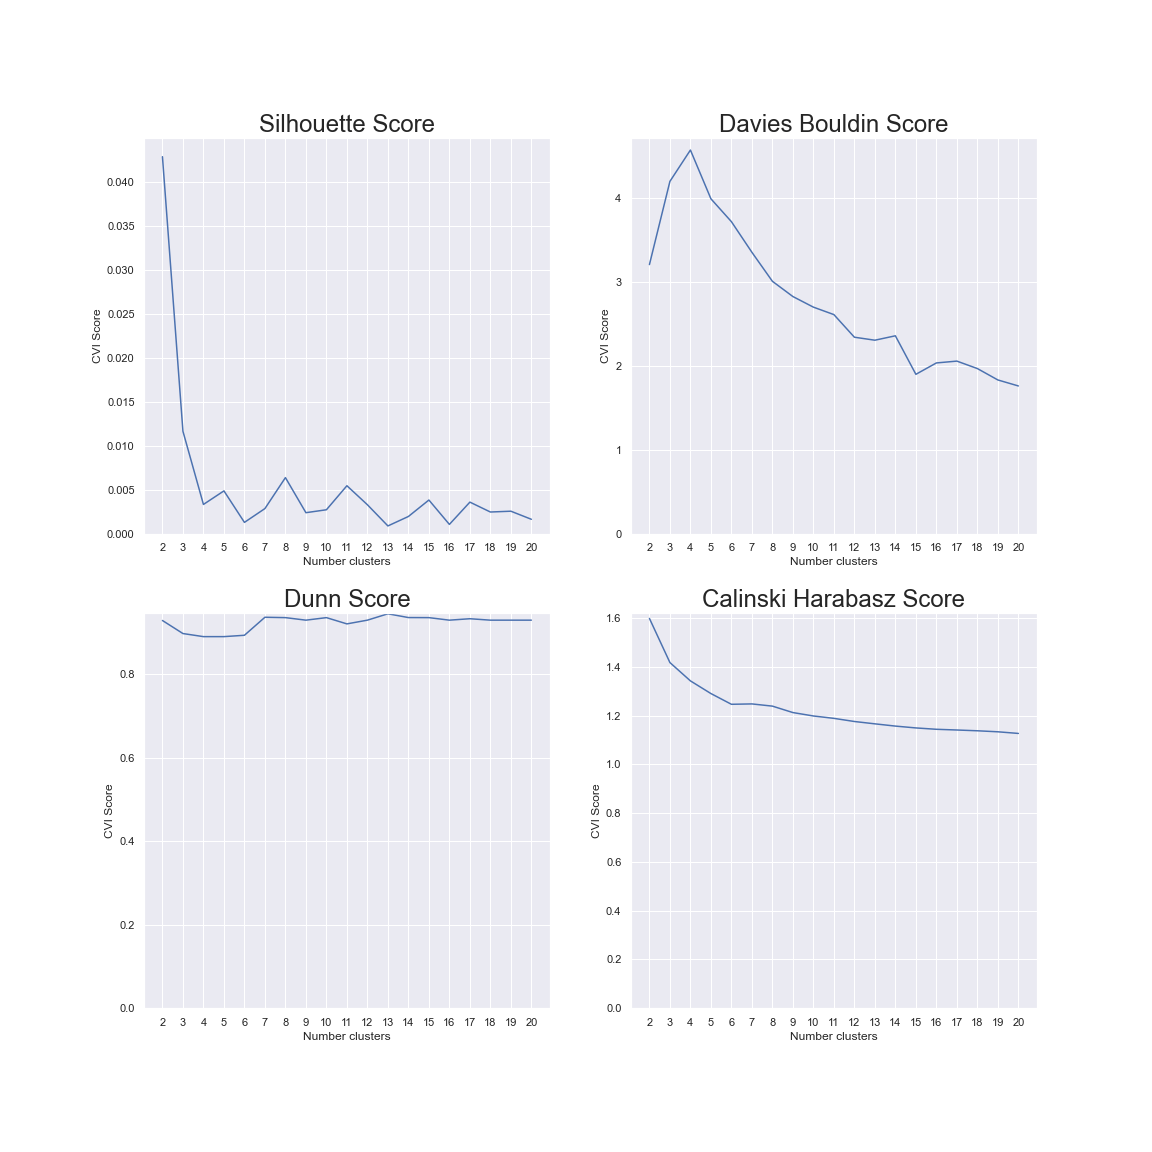
\includegraphics[width=0.9\textwidth]{ncd_cvis.png}
	\caption{CVI Functions of NCD}
	\label{fig:cvi_ncd}
\end{figure}



\clearpage
Considering the "elbow" in the Calinski Harabasz and the slight peaks in figure \ref{fig:cvi_ncd_combo}, eight was chosen for the number of clusters.

\begin{figure}[h!]
	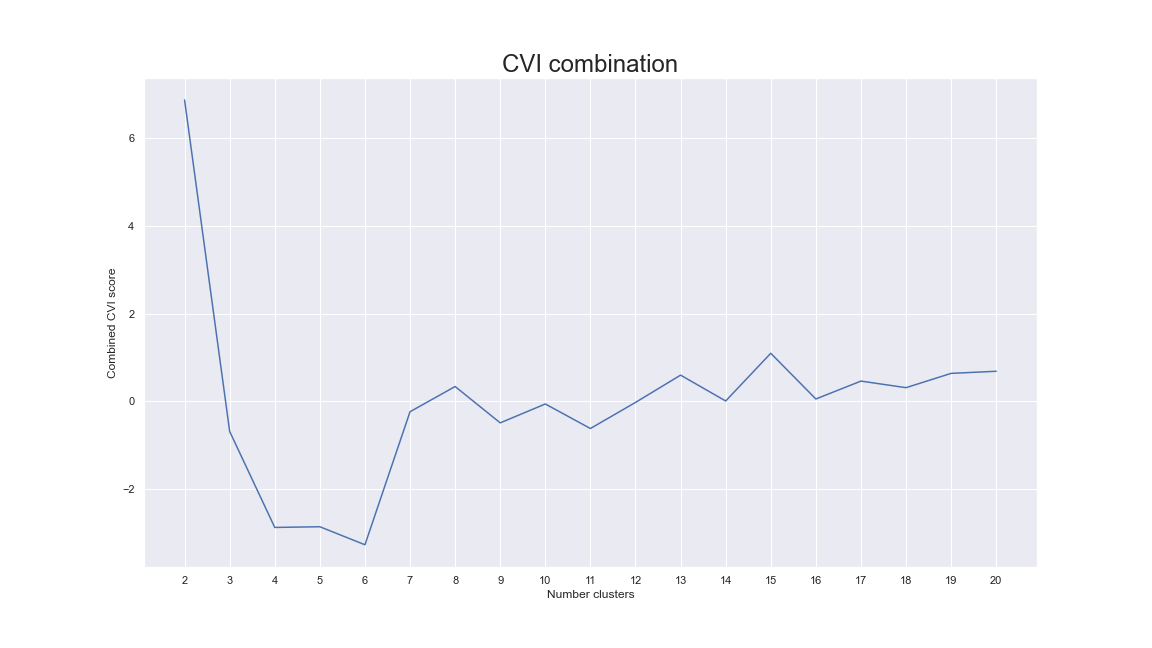
\includegraphics[width=1\textwidth]{cvi_combination_ncd.png}
	\caption{CVI Combination (NCD)}
	\label{fig:cvi_ncd_combo}
\end{figure}



\clearpage
Figure \ref{fig:ncd_clusters} shows the outcome of the k-Means algorithm using 8 clusters.

Interestingly for the first time all synthetic generated time series (ggggg 1 to 4) were clustered in the same cluster (\#6).

\begin{figure}[h!]
	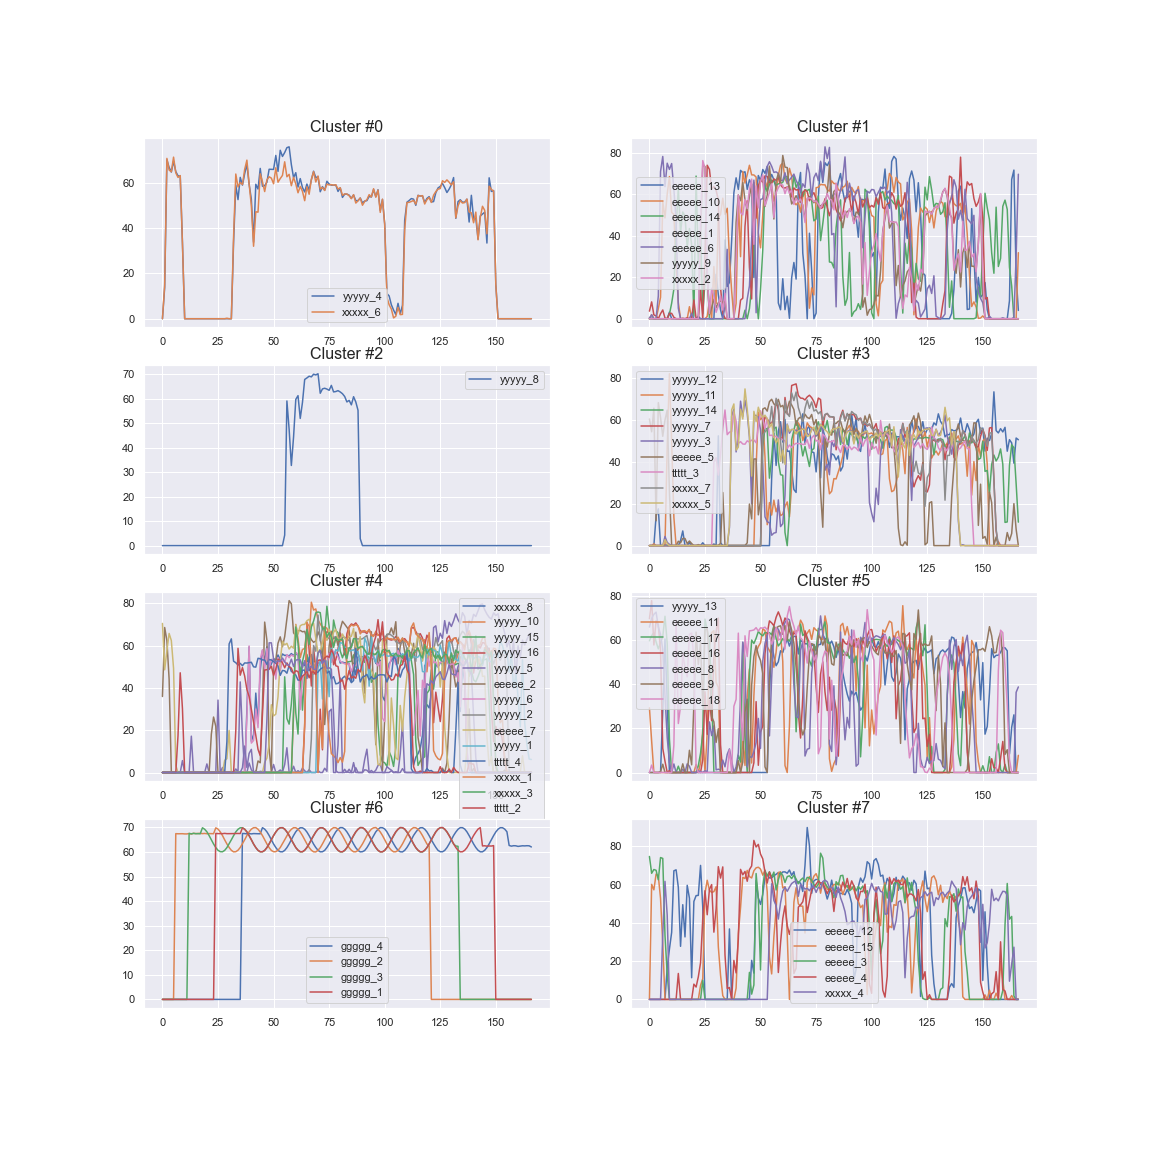
\includegraphics[width=1.1\textwidth]{ncd_clustering.png}
	\caption{Clusters (NCD)}
	\label{fig:ncd_clusters}
\end{figure}

